\chapter{Post-Compromise Security} \label{ch:postcomp}
%Intro
Intro\\compromise window\\
\par
ratchet key exchange (RKE) URKE, SRKE, BRKE
\par
“a ratcheting
forward secrecy protocol that works in synchronous and asynchronous messaging environments” [55, 56].
Signal’s goals include end-to-end encryption as well as advanced security properties such as perfect forward secrecy and “future secrecy”
The Signal protocol can be roughly divided into three types of stages:
• The initial key exchange, or X3DH (extended triple Diffie-Hellman) protocol [64], which combines
long-term, medium-term and ephemeral Diffie-Hellman keys to produce a shared secret “root” value.
• An asymmetric ratchet stage [63], where users alternate in sending new ephemeral Diffie-Hellman keys in a ping-pong fashion with previously generated root keys to generate forward-secret chaining keys.
• A symmetric ratchet stage [63], where users take no additional entropy but instead use key derivation
functions to ratchet forward chaining keys to create symmetric encryption keys.

\section{\acrfull*{x3dh}}
\textbf{\LARGE \# FIXME intro \#}
\label{ch:x3dh}

Key establishment protocols are utilized by communicating parties to establish shared secrets, in some cases, with the aid of a trusted third party \cite{handbookOfAppliedCrypto}. As per \cite{handbookOfAppliedCrypto}, key agreement is a key establishment technique in which a shared secret is derived by parties as a function of information related to them, such that the secret in not predeterminable nor deducable by outsiders.
\par
The Security of protocols is required to be proven to avoid the devastating effects of malicious attacks. Therefore, verification of security protocols is a vital process. Verification is proving that a protocol model is secure by achieving a set of security goals. There are various model checking tools that provide verification.
\par
\gls{x3dh} is a key agreement protocol intended for asynchronous settings \cite{x3dh}. The protocol can establish a shared secret between two parties in an environment where it is recurring that one of the parties is offline and the other wishes to send it an encrypted message. Also, X3DH provides the desired feature of forward secrecy. 
\par
This chapter discusses the \gls{x3dh} key agreement protocol \cite{x3dh} and verifies the security of the protocol using \gls{ofmc} \cite{ofmc}.
\subsection{Protocol Overview}
\subsubsection{Roles}
A protocol run involves three roles: Alice, Bob, and a server. In this description, Alice wants to send an encrypted message to Bob. Bob is the party that may be offline at that time and wishes to enable other parties to derive a shared secret with it, through a set of public information Bob publishes. The server is responsible for 1. storing the public information published by Bob, and 2. storing messages for offline parties till they are fetched. The server is not trusted, however, it is assumed to be resilient against DoS. % more details.
\subsubsection{Keys}
\gls{x3dh} utilizes Elliptic Curve asymmetric key pairs. All keys used in a protocol run must all be derived from the same curve, either $X25519$ or $X448$. Each role has to have a set of keys to run the protocol. Table \ref{tab:x3dhkeys} lists the public keys required for each role. Note that for each public key, there exists a corresponding private key at its owner.

\begin{table}
	\centering
	\begin{tabular}{|c||c|c|}
		
		\hline
		Owning Role & Notation				 & Description 			  \\\hline
		\multirow{2}{*}{Alice} & IK\textsubscript{A} 	 & Long-term identity Key \\
		& EK\textsubscript{A} 	 & Ephemeral Key 		  \\\hline
		\multirow{3}{*}{Bob}  & IK\textsubscript{B} 	 & Identity Key 		  \\
		& SPK\textsubscript{B} 	 & Signed Prekey 		  \\
		& OPK\textsubscript{B} 	 & one-time Prekey 		  \\ \hline
		
	\end{tabular}
	\caption{\gls{x3dh} keys.}
	\label{tab:x3dhkeys}
\end{table}

\begin{itemize}
	\item \textit{Identity keys}: They are long-term public keys known by their corresponding parties before the protocol run.
	\item \textit{Ephemeral Keys}: This type of key pair is freshly generated within the protocol run.
	\item \textit{Signed Prekey}: This key pair is generated and signed by its owner. The prekey is signed using the private identity key. The life time of this key pair is shorter than that of the identity key pairs as it is updated periodically by its owner. The corresponding role owns only one signed prekey at a time.
	\item \textit{One-time Prekey}: The corresponding role generates multiple one-time prekey. Each is can be used for only one protocol run. The responsible party is supposed to supply the these keys as they should not run out. In case there are not any keys left, the protocol can run, however without one of the \gls{dh} operations as explained in section 2.3.
\end{itemize}

\subsubsection{A Protocol Run}
%\subsubsubsection{Registration phase} 
At first, the protocol starts with a registration phase. Initially, The party acting in the role of Bob publishes to server the public information required to run the protocol with it by any party acting as Alice. Bob publishes his $ IK_{B} $, $ SPK_{B} $, Bob's prekey signature, and a set of $ OPK_{B} $.

\par
%\subsubsubsection{The initial message}
Next, the inline party sends the initiates the protocol by sending the first message. First of all, Alice fetches a \textit{prekey bundle} from the server to contact Bob. This bundle contains:
\begin{itemize}
%	\setlength\itemsep{-0.3em}
	\item Bob's Identity key $ IK_{B} $.
	\item Bob's signed prekey $ SPK_{B} $.
	\item Bob's prekey signature.
	\item If exists, a one-time prekey $ OPK_{B} $. The server deletes the $ OPK_{B} $ sent to Alice.
\end{itemize}

Before proceeding, Alice verifies the prekey signature and quits the protocol if the verification fails.
At this point, Alice has enough information from Bob to deduce a shared secret. Alice generates her Ephemeral key pair $ EK_{A} $. With the set of available keys, Alice performs three \gls{dh} operations which are extended to four if a $ OPK_{B} $ is available. Figure \ref{fig:x3dh} presents the relation between the keys.

\begin{itemize}	
\item $ DH1 = DH(IK_{A_{p}} \footnote{\textit{p} indicates the private key of the key pair.}, SPK_{B}) $
\item $ DH2 = DH(EK_{A_{p}}, IK_{B}) $
\item $ DH3 = DH(EK_{A_{p}}, SPK_{B}) $
\item \textcolor{darkgray}{$ DH4 = DH(EK_{A_{p}}, OPK_{B}) $}
\end{itemize}

\begin{figure}[htbp]
	\centering
	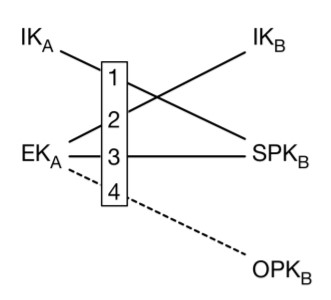
\includegraphics[width=0.4\linewidth]{images/X3dh}
	\caption{\gls{x3dh} operations \cite{x3dh}.}
	\label{fig:x3dh}
\end{figure}

The \gls{dh} outputs are fed into a \gls{kdf} to generate the shared secret $ SK $. Next, Alice deletes her $ EK_{A_{p}}$ and all \gls{dh} outputs for forward secrecy. At this moment, Alice is ready to send the initial message with the content encrypted using $ SK $. The initial message from Alice to Bob has to have enough information for Bob to generate the same $ SK $.
The initial message contains:
\begin{itemize}
%	\setlength\itemsep {-0.3em}
	\item $ IK_{A} $
	\item $ EK_{A} $
	\item Identifiers of Bob's prekeys used by Alice
	\item An initial ciphertext. The ciphertext can be used as an initial message for a post-X3DH communication protocol, e.g. Double Ratchet algorithm.
\end{itemize}

%\subsubsubsection{Bob's $ SK $ Derivation}
Upon receiving the initial message, Bob attempts to derive the $ SK $.
Using the key identifiers sent by Alice, Bob loads the private keys corresponding to the public keys Alice used. In combination with the keys $ IK_{A} $ and $ EK_{A} $ Alice sent, Bob can compute the same $ SK $ by doing the three (or four) \gls{dh} operations.
\par
Next, Bob attempts to decrypt the ciphertext. If the message is successfully decrypted to the expected format, e.g. the format of the first message of the post-X3DH protocol, then the protocol run was successful. Otherwise, Bob aborts the protocol and discards the $ SK $.

\subsubsection{Security Considerations}
%\subsubsubsection{Authentication}
Authentication is essential for both parties to guarantee the identity of who they are communicating with. Thus, Alice and Bob must authenticate the keys $ IK_{A} $ and $ IK_{B} $. However, the protocol specification does not discuss authentication methods.
\par
%\subsubsubsection{Protocol Replay}
The one-time prekey used in the fourth and optional \gls{dh} calculation is for protection against replay attacks as they ensure freshness of the protocol run. Absence of a one-time prekey could lead a replayed message to be accepted by Bob believing that Alice had sent it in the current protocol run.
\par
%\subsubsubsection{Server Trust}
A server can be a cause of attacks if malicious. It can carry out a Denial of Service attack if it refuses to forward the messages. It can deliberately not distribute one-time prekeys, exposing the protocol to replay attacks. Also, one party can drain all the one-time prekeys, if the server is not attentive to such action, leading to replay attacks.

\subsection{OFMC Verification}
This section aims at formally verifying the \gls{x3dh} protocol using the automated verification tool \gls{ofmc}. Briefly, \gls{ofmc} uses the clear and declarative modeling language $AnB$. The goal of the tool is verify the security of the modeled protocol, under an intruder model, in a fashion similar to deciding whether a mathematical statement is true or false. The intruder model is based on the famous Dolev-Yao model \cite{dolev1983security}. The intruder is assumed to control the network. Therefore, the network should not be relied on for any protection guarantees. Furthermore, the intruder is assumed to be knowledgeable to all cryptographic primitive. Lastly, \gls{ofmc} does not rule out the possibility that the protocol participants can be dishonest.

Presented in listing \ref{model} the code for modeling our variant of a secure \gls{x3dh} protocol under the Dolev-Yao intruder model in \gls{ofmc} using the \textit{AnB} language.

\lstinputlisting[numbers=left,          
numberblanklines=false, breaklines=true, columns=fullflexible,
frame=single,
breaklines=true,
postbreak=\mbox{\textcolor{red}{$\hookrightarrow$}\space},
caption={X3DH \gls{ofmc} Model},captionpos=b, label={model}]{code/x3dh.anb}

\subsubsection{Types section} 
Here, the parameters of the protocol are defined, e.g. variables, constants, roles, etc. Line 4 defines the participants of the protocol of type \textbf{Agent}.
\begin{itemize}
	\item $A$ and $B$: Variables indicating Alice and Bob. A variable may be dishonest in an \gls{ofmc} protocol run.
	\item $s$: Constant indicating the server. Constants act as trusted third parties.
\end{itemize}
\par
Line 5 defines the functions of the protocol.
\begin{itemize}
	\item $kdf$: Key derivation function.
	\item $pk$: A function to model asymmetric key pairs. A public key for Alice is modeled as $pk(A)$ and the corresponding private key is computed using the internal function $inv()$ as follows $inv(pk(A))$.
	\item $ik$: models the private component of the identity key of a party for the \gls{dh} calculations.
\end{itemize}
	Alice and Bob have long-term signing keys modeled by the function $pk()$ and long-term identity keys modeled by the function $ik()$.
	\par
Line 6 defines the numbers used in the protocol. Lower-case numbers are constants, while upper-case numbers are random and freshly generated during a protocol run. Some private components of keys are modeled as numbers as they are required to be freshly generated during a protocol run which can not be done using functions.
\begin{itemize}
	\item $g$: Public prime base for \gls{dh} calculations.
	\item $NA$: Alice's Nonce.
	\item $EKA$: The private component of Alice's Ephemeral key.
	\item $OTP$: The One-time prekey's private component.
	\item $PREKEY$: the prekey's private component.
	\item $MSG1$ and $MSG2$: Random numbers used as placeholders for random and fresh messages.
\end{itemize}

\subsubsection{Knowledge section}
This section of the model defines what knowledge is initially known to each party before the protocol starts. Line 9 defines Alice's knowledge which contains, in addition to the previously defined parameters, Alice's certificate modeled as $\{A, pk(A)\}inv(pk(s))$. This translates to Alice's identity $A$ and Alice's public key $pk(A)$ are signed using the servers private key $inv(pk(s))$. 

Line 15 holds a $where$ clause that strictly defines $A$ and $B$ as different parties to avoid the scenario where $A$ or $B$ talk to itself.
\subsubsection{Actions section}
The Actions section states the protocol's message sequence between the participating parties for a successful protocol run. Throughout this section messages are referred to according to their line number, e.g message 19 is the message in line number 19 of the model code.
\par
Message 19 represents the registration phase where Bob publishes his public information to the server. The whole message is encrypted for authenticity by the server's public key $pk(s)$. The message contains the following:
\begin{itemize}
	\item $exp(g,Z)$: The public \gls{dh} key of the corresponding private key Z. As known in \gls{dh}, the public key of a party is of the form $g^{Z}\ mod\ p$. For simplicity, \gls{ofmc} omits the prime modulus operation $mod\ p$. Hence, it is needed to only model the public key $g^{Z}$ by using the \gls{ofmc} modulus exponentiation function $exp(g,Z)$.
	\item $\{exp(g,PREKEY)\}inv(pk(B))$: The prekey of Bob signed by Bob's signing key.
\end{itemize}

\par
Message 21 is not an actual part of the protocol, however, it is included for the sake of modeling the protocol with the chosen tool. This is because of the asynchronous communication model of \gls{ofmc} and the strands concept \cite{ofmcTut}.
\par 
In message 23, Alice requests to fetch from the server a key bundle to communicate with Bob. A nonce $NA$ is attached for freshness.
\par
Message 25 is the server's response to Alice's key bundle request. The message contains the requested key bundle required to communicate with Bob, as well as Alice's nonce. The whole message is integrity protected by the server's signature.
\par
Message 27 represents the initial message from Alice to Bob. It is composed of the following:
\begin{itemize}
	\item (Line 27) Alice's certificate for authenticity.
	\item (Line 29) Bob's keys that Alice received from the server which will used to compute $SK$. All these keys are signed by Alice for integrity protection.
	\item (Line 31) The initial ciphertext encrypted by the symmetric key $SK$. Each output of the four \gls{dh} operations is input into the \gls{kdf} resulting in $SK$.
\end{itemize}
Message 38 is the last message of the protocol run. Here, Bob shows he is able to compute the same $SK$. 
\par
Notably, the modeling of the \gls{dh} operations in messages 27 and 38 is unnatural in contrast to how \gls{dh} is normally performed. Ordinarily, a \gls{dh} secret is the computation of $exp(g^{M},N)$ where $g^{M}$ is a public value and $N$ is a value private to the party performing the operation. According to exponential power of power rule $exp(g^{M},N)$ is equivalent to $exp(g^{N},M)$. Therefore, the other party should follow that intuition to result in the same secret output as its counterpart. 
It is observable that the symmetric key computation in message 27 is identical to the one in message 38.
The behavior for modeling $DH1$, $DH2$, and $DH3$ of message 27 is not expected, since Alice is explicitly using Bob's secrets ($PREKEY$ and $ik(B)$) in the \gls{dh} operations although they ought not be in Alice's knowledge.
This behavior is present in message 38, however, it is as it should be. To the reader, it could mean that Alice is knowledgeable of Bob's private keys, but, this is not the case. \gls{ofmc} aims to abstract the key creation process and makes it implicit for the tool users. The \gls{ofmc} compiler comprehends the exponential power of power property which enables it to automatically do the computation. Despite the previous clarification, $DH4$ computation contradicts what was mentioned. The $M$ and $N$ values for $DH4$ are swapped back to what would be naturally expected in comparison to the previous \gls{dh} operations of message 27. Although, this behavior is considered unnatural for message 38 as now Bob is considered to be using Alice's secret keys. However, this exceptional behavior for $DH4$ is a result of a limitation of \gls{ofmc}'s AnB-translator message composition heuristics, as the translator is not capable of recognizing four inversions in a row. Therefore, the exceptional behavior is a workaround to make the AnB-translator realize how to compose the message. This workaround was thankfully guided by Prof. M\"{o}dersheim, the composer of \gls{ofmc}.
\subsubsection{Goals section}
This section of the model lists the security goals which the protocol must achieve at the end of a run. There are two types of goals
\begin{itemize}
	\item Authenticity: When a party wants to make sure a certain message has been generated and sent by the other party. In this model, Alice and Bob authenticate each others' public keys. Bob authenticates the server on the keys he received in message 27 from Alice, to be sure that the keys are forwarded by Alice from the server without tampering.
	\item Secrecy: The requirement for a message to be secret only between some parties.
\end{itemize}
\subsubsection{Deviations from specification}
\begin{itemize}
\item \textbf{Registration Phase:} The specification was not specific about how to securely publish Bob's keys to the server and the security of the connection between the server and the communicating parties. Therefore, the registration message from Bob to the server is encrypted by the server's public key.
\item \textbf{Use of Signatures:} The specification discouraged the use of signatures as they reduce deniability which is a desired feature in the messaging application setting which the protocol is intended for. However, this model used signatures.
\begin{enumerate}
	\item Signature are used in responses from the server to assure integrity of messages to receivers.
	\item Alice and Bob have an additional key pair for signing other than the identity key pairs. They are used to sign parts of messages which were vulnerable to attacks by intruders and would break the protocol's security. For example, Bob's keys which Alice used to compute $ SK $ in message 27.
\end{enumerate}
\item \textbf{Use of Certificates:} Alice used a certificate signed by the server to authenticate itself in-band as opposed to the specification which ruled the authentication between the parties as a necessary but out of scope operation.
\end{itemize}
%\subsubsection{Result}
result of formal verification.





\section{Double Ratchet Algorithm}
\label{ch:dr}
The adoption of a ratchet mechanism is a popular mechanical approach that enables forward movement but inhibits backward movement. A ratchet-like action is performed in the context of secure communication by utilizing randomization in every state update, such that a compromised state is insufficient for the decryption of any subsequent transmission.
The Double Ratchet is a cryptographic asynchronous message exchange algorithm that provides high security to the communicating parties. Asynchronicity in this context refers to that even if the counterpart is not online, the messages should be conveyed (or the key exchange should be done) for a two-party conversation.
Furthermore, a significant design goal dubbed \gls{0rtt} is the ability to transfer payload data without necessitating online exchanges.
\par
The algorithm enables the exchange of encrypted messages based on a shared secret key between the two parties where each message is encrypted with its specific ephemeral key.
The double ratchet algorithm is a combination of two ratchet constructions which provide enhanced security properties.
The first outer ratchet is inherited from \gls{otr}'s asymmetric ratchet to benefit from its future secrecy property which is obtained through the use of ephemeral key exchanges. Coupled by an inner symmetric ratchet for forward secrecy, the algorithm was formed and was formerly named Axolotl Ratchet. Additionally, \gls{kdf} chains are a core concept of the algorithm. This section goes through the methodology of the algorithm, its features, and its security properties.

\subsection{\gls*{kdf} Chain}
As mentioned in section \ref{backgroung:kdf}, a \gls{kdf} is a function that takes as input a key and an input and produces a cryptographically secure hash output that is random-like.
A \gls{kdf} chain is a series of connected \gls{kdf}s where one output key of a \gls{kdf} is a \gls{kdf} key input of a succeeding \gls{kdf}. Figure \ref{fig:kdf-chain} shows an illustration for a \gls{kdf} chain that takes three external inputs and produces three random output keys.

\begin{figure}[hptb]
	\centering
	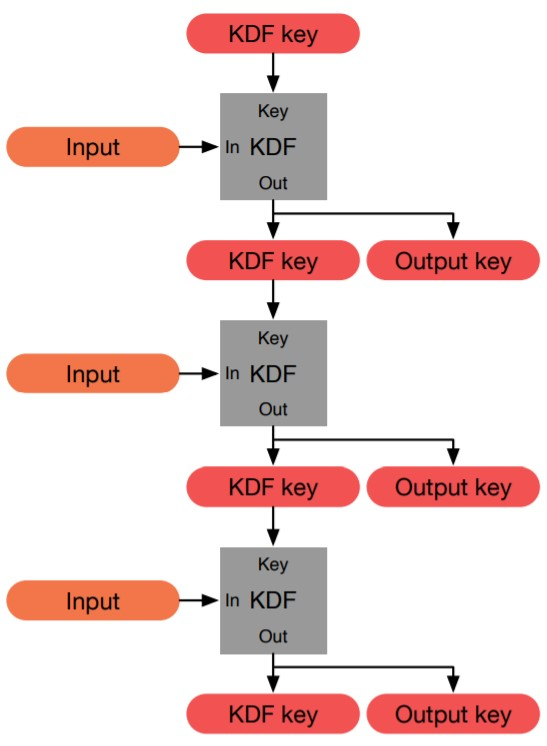
\includegraphics[scale=0.4]{Images/kdf-chain.jpg}
	\caption{A 3 input KDF chain \cite{dblRtcht}.}
	\label{fig:kdf-chain}
\end{figure}

The algorithm session has three \gls{kdf} chains: root chain, sending chain, and receiving chain. Each chain is advanced whenever its relevant ratchet performs a step. More details about ratchet steps and their relation to the \gls{kdf} chains are discussed in later sections.
\par
KDF chains have a set of characteristics \cite{dblRtcht}:
\begin{itemize}
	\item \textit{Resilience:} An adversary who does not know the KDF keys perceives the output keys as random. Even if the opponent has complete control over the KDF inputs, this is still valid.
	
	\item \textit{Forward secrecy:} An adversary who discovers the KDF key at some point in the future cannot distinguish between past output keys and random.
	
	\item \textit{Future secrecy:} If future inputs have contributed adequate randomness, future output keys seem random to an adversary who learns the KDF key at some point in the future.
\end{itemize}

\subsection{Symmetric-key Ratchet}
	
The sending and receiving chains are constructed of symmetric-key ratchets where Alice's sending chain is equivalent to Bob's receiving chain and vise versa. Essentially, a symmetric-key ratchet is a \gls{kdf} chain with a constant input through out the chain steps. However, unlike with random input, a constant input does not provide future secrecy.
\par
In a symmetric-key ratchet, the KDF key illustrated in figure \ref{fig:kdf-chain} is the chain key, while a KDF's output key is a unique message key. For a sending chain, a message key is used to encrypt the outgoing message. On the other side, a message key in the receiving chain is used to decrypt the incoming message. The process of calculating the next chain and message keys is an advance in the sending/receiving chain. This is referred to as a \textit{symmetric ratchet step}.
\par
Message keys are not re-introduced into the KDF chain, therefore, they can be discarded without proposing any security risk to earlier or later ratchet outputs. Also, it is possible to store message keys to handle out-of-order messages on the receiving end. Storing message keys introduce a risk to only their respective messages. However, a compromise of a chain key can lead to further compromise of future chain keys as future chain keys rely on previous ones.

\subsection{Diffie-Hellman Ratchet}
The \gls{dh} ratchet provides the future secrecy property. When paired with the symmetric ratchet, the combination addresses the symmetric ratchet lack of future secrecy. 
Each party generates a \gls{dh} key pair known as their \textit{ratchet key pair}. The parties exchange their public keys within message headers with which each can compute an equivalent \gls{dh} secret output using their own private key that is equivalent to the public key they sent. The process of generating a new \gls{dh} output when receiving a new public key is referred to as a \textit{\gls{dh} ratchet step}. Accordingly, a passive adversary that compromises one party's private key at a point in time is incapable of deducing the upcoming \gls{dh} outputs due to the use of newly generated key pair for each ratchet step.
\par
Next, we discuss an algorithm run where a \gls{dh} ratchet is advanced to create two different DH secret outputs between Alice and Bob. Bob is assumed to be the algorithm initiator. Figure \ref{fig:dh-bobRatchet} serves as visual aid for our discussion where we proceed in steps as labeled in the diagram.

\begin{figure}[hptb]
	\centering
	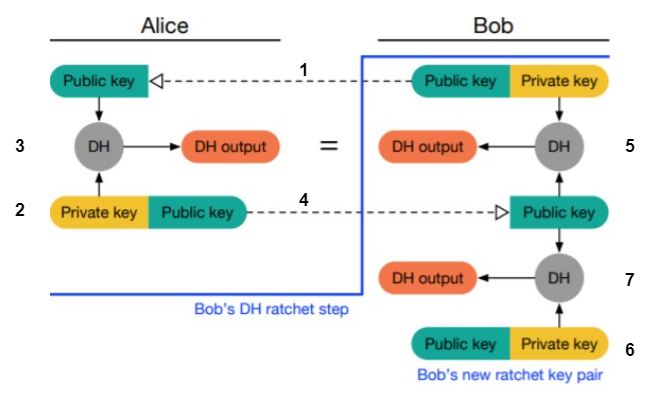
\includegraphics[scale=0.45]{Images/dr-bobRatchet.png}
	\caption{Bob \gls{dh} Ratchet step. Figure reproduced from \cite{dblRtcht}.}
	\label{fig:dh-bobRatchet}
\end{figure}

\begin{itemize}
	\item \textit{Step 1:} Bob generates his first ratchet key pair to send the initial message to Alice. The initial message contains Bob's public key. 
	
	\item \textit{Step 2:} Upon receiving Bob's public key, Alice generates her ratchet key pair.
	
	\item \textit{Step 3:} Alice performs a \gls{dh} calculation between her private key and Bob's public key generating her side of the DH output.
	
	\item \textit{Step 4:} Alice advertises to Bob her public portion of her ratchet key pair that was used to generate the DH output.
	
	\item \textit{Step 5:} After obtaining Alice's ratchet public key, Bob performs a DH calculation between it and his current ratchet private key resulting in Bob's copy of the shared DH output.
	
	\item \textit{Step 6:} Furthermore, Bob generates a new ratchet key pair to generate the next DH output.
	
	\item \textit{Step 7:} Bob performs a \gls{dh} calculation between hit new ratchet private key and Alice's public key generating a new DH output.
\end{itemize}
The steps described above are Bob's DH ratchet step as Bob was the initiator of the ratchet step by advertising his public key. Similarly, Alice's ratchet step starts by sending her public key to Bob and concludes after performing the same steps mentioned above but with the roles reversed.
\par
Linking the algorithm to the messaging context, the DH outputs represent the sending and receiving chains' root keys. 
Each party need to have two chains, sending and receiving chains. Alice's sending chain is equivalent to Bob's receiving chain and vice versa. As depicted in figure \ref{fig:dh-chains}, when a party receives a public key and computes its chain key using a private key that was generated prior to receiving the public, the resulting chain key is the receiving chain key. However, if they private key is generated after receiving the public key, the resulting key is the sending chain key. Simply put, if the public key is used in a DH operation upwards it produces a receiving chain key, while using it in a downwards DH operation generates a sending chain key.
\begin{figure}[hptb]
	\centering
	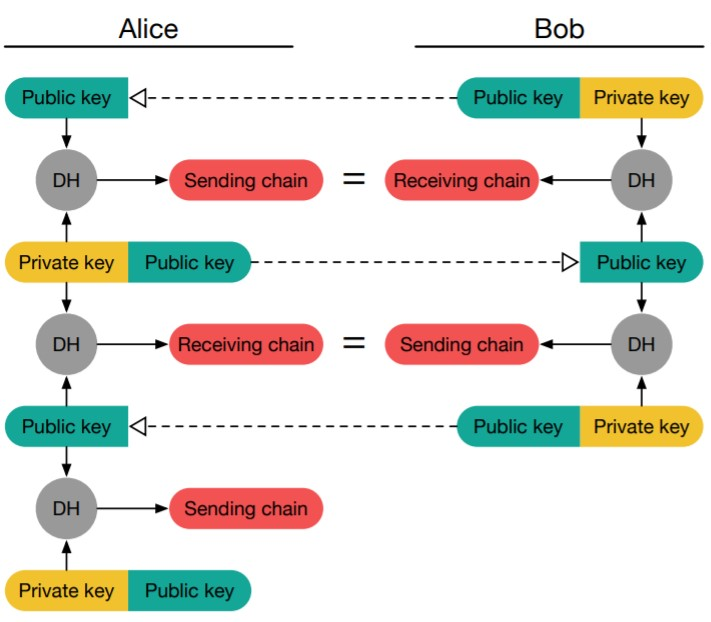
\includegraphics[scale=0.5]{Images/dh-chains.jpg}
	\caption{\gls{dh} chain keys generation \cite{dblRtcht}.}
	\label{fig:dh-chains}
\end{figure}
\par
However, the description so far is simplified. The algorithm is augmented by a KDF chain to improve resilience and future secrecy. The KDF chain key is a shared secret between both parties while the KDF inputs are the DH outputs from the DH ratchet. Every step through the KDF chain results in a new KDF root key and a sending/receiving chain root key. So a full DH ratchet step consists of updating the root KDF chain twice, generating both a sending and a receiving chain key. Figure \ref{fig:dh-ratchet_chain} illustrates a full DH ratchet step.

\begin{figure}[hptb]
	\centering
	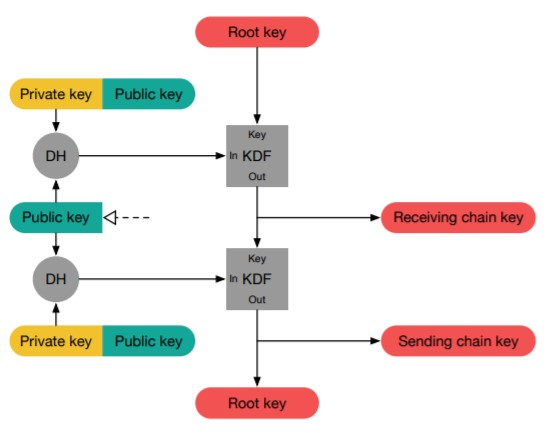
\includegraphics[scale=0.65]{Images/fullDHRatchetStep.jpg}
	\caption{A full \gls{dh} Ratchet step \cite{dblRtcht}.}
	\label{fig:dh-ratchet_chain}
\end{figure}

\subsection{Double Ratchet}
The double ratchet combines both the symmetric-key ratchet and the \gls{dh} ratchet to merge the security advantages provided by each. The outer ratchet is the \gls{dh} ratchet that provides ephemeral DH outputs which improve future secrecy. The DH outputs are fed as inputs to a KDF root chain lying between the outer and inner ratchets. It contributes to augmenting the security features by providing resilience and forward secrecy to the generated keys. The initial \gls{rk} for the KDF chain is a shared secret between the parties, e.g. an output of a key agreement protocol. The KDF chain outputs a new \gls{rk} for the next KDF and a new root \gls{ck} to create a new sending/receiving chain. Lastly the inner ratchet is the symmetric-key ratchet. Their root chain keys are the \gls{ck}s generated from the previous layer. They form the sending and receiving chains. When this ratchet is advanced it generates a new \gls{ck} and a message key. The \gls{ck} is used in the next KDF and the message key is used to encrypt or decrypt the message, depending on its respective chain. 
\par
Figure \ref{fig:AliceDR} serves as an example scenario for an algorithm run as it illustrates Alice's perspective of her double ratchet algorithm after a series of steps. 
\begin{figure}[hptb]
	\centering
	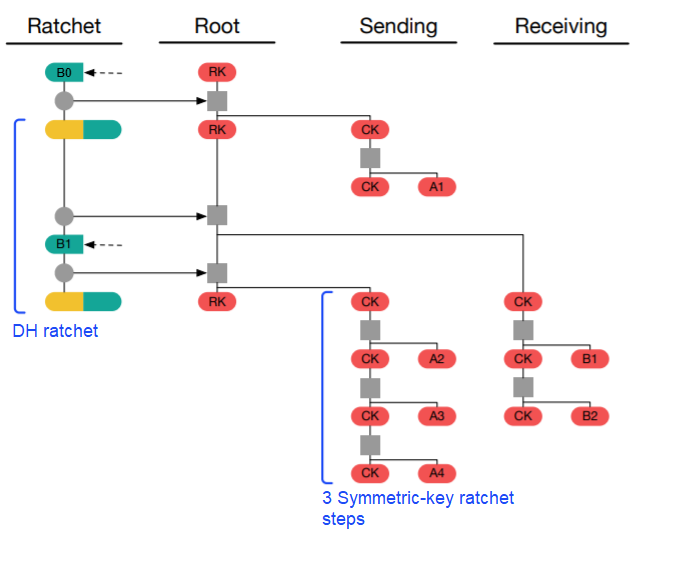
\includegraphics[scale=0.48]{Images/dr.png}
	\caption{Double ratchet from Alice's point of view. Figure reproduced from \cite{dblRtcht}.}
	\label{fig:AliceDR}
\end{figure}
The figure is split into four columns describing the aspects of the algorithm and how they are connected to each other. The first column represents the DH ratchet, the second shows the root KDF chain, and the last two depict the sending and receiving symmetric-key ratchets. Messages are denoted by the initial of the sender and the number of the message, e.g. $A1$ denotes Alice's first message. Keys follow the same abbreviation convention, e.g. $B1$ denotes Bob's first message key. Whether the key is a public key or a message key is represented by their highlighted color. Message keys are highlighted in red while public keys are highlighted in green.
\par
Alice is initialized by receiving the initial public key $B1$ which she uses to compute the input for the root KDF chain through a DH operation. Along with the pre-shared \gls{rk}, Alice computes a root \gls{ck} for her sending chain and a new \gls{rk}. Using the initial \gls{ck}, Alice creates a sending chain by performing a symmetric-key ratchet and producing a new \gls{ck} and a symmetric key $A1$ that she uses to encrypt her first message to Bob.
\par
Till this point, Alice is able to send encrypted messages to Bob as it had created her sending chains. However, she cannot decrypt Bob's messages as she has not yet created a receiving chain to produce the keys required to decrypt Bob's messages. As soon as Bob sends his next message with a new public key, Alice uses the public key $B1$ attached in the message header to step her DH ratchet. $B1$ is used in a DH operation with the previously created key pair to ultimately produce a root \gls{ck} to create a receiving chain. Alice performs a symmetric-key ratchet step of her receiving chain to produce the symmetric key $B1$ that decrypts the received message. Alice advances the same receiving chain to produce message keys to decrypt further message from Bob, e.g. $B2$, as long as the received messages do not contain new public keys in the message headers. However, since Alice received $B1$ and had to perform a full DH ratchet step, she has to generate a new ratchet key pair ultimately create a new sending chain. This implies if Alice wishes to send further encrypted message, she must use the new sending chain to generate the new message key. Thus in figure \ref{fig:AliceDR}, $A2$ is produced from the newly generated sending chain not the old one. As long as Alice has not received a new public key, she keeps advancing the sending chain to generate encryption keys for her outgoing messages, e.g. $A2$ and $A3$ in figure \ref{fig:AliceDR}.
\par
Parties should delete old keys as they no longer have a use. Keys are considered old if they have already been used and they are not going to be used in the future. For example, \gls{rk}s and \gls{ck}s which have already been input into KDFs or message keys that have already been used to encrypt/decrypt messages are considered old keys. Deleting old and useless keys is a good security practice as it prevents intruders from the possibility of recomputing keys that are dependent on those keys. Nevertheless, some keys can be saved to support additional functionalities such as handling out-of-order messages as explained in section \ref{oooMsgs}.

\subsubsection{Out-of-order Messages}\label{oooMsgs}
The Double ratchet algorithm can manage messages arriving out-of-order by simple additions to the message headers from the sender side. By including the message's index $N$ ($N=0$ for message 1) in the sending chain and the length $PN$ of the previous sending chain.
\par
If the sent message does not trigger a DH ratchet step on the receiver side, then the out-of-order message belongs to the current receiving chain of the receiver. The difference between $N$ and the actual receiving chain length is the number steps the receiver has to advance his receiving chain to obtain the message key required to decrypt the received message. The intermediate message keys for the skipped messages are stored in case they arrive later.
\par
On the other hand, if the message triggers a DH ratchet step, then the receiver uses the $PN$ to determine how many messages are skipped of his current receiving chain. The difference between the current length of the chain and $PN$ is the number of steps needed to advanced in the current chains and their produced message keys have to be saved. In this case, $N$ determines the number of skipped messages in the new receiving chain after advancing the DH ratchet. Likewise, the message keys for the skipped messages have to be saved supposing they are delayed for any reason.
\par
Implementation wise, the algorithm defines a \textit{MAX\_SKIP} constant that specifies the maximum number of message keys that should be saved for skipped messages. It should tolerate message loss or delay. However, it should not be too high that it allows for a malicious sender to trigger excessive recipient computation.
\subsubsection{Header Encryption}
As headers contain ratchet public keys as well as $PN$ and $N$ values, a passive attacker can infer the ordering of messages inside a session, or which messages belong to particular sessions. Therefore, encrypting message headers can reinforce messages security. Header encryption is achievable through each party having symmetric keys for both sending and receiving chains to encrypt or decrypt messages' headers. One chain header key is responsible for handling the header encryption of all messages within its respective chain. The header keys are integrated into the double ratchet algorithm as follows.
\par
Originally, Alice and Bob had only one pre-shared secret, the \gls{rk}. To integrate header encryption, the initial shared secrets need to include two unique \glspl{hk}, one for the sending chain and the other for the receiving chain (referred to as \acrfull*{nhk} in \cite{dblRtcht}). The initial \glspl{hk} are used for their respective first generated chains of the algorithm. To continuously obtain new \glspl{hk} for the newly generated chains which are a result of advancing the  DH ratchet, the root KDF chain is amended. Instead of generating only a new \gls{rk} and a new respective \gls{ck} with each step, the root chain is modified to additionally produce a \gls{nhk} of the relevant chain. A \gls{nhk} is a \gls{hk} that is to be used for the next chain of the same type that is to be generated after the next ratchet step. In this manner, at any point in time, before generating any chain of the algorithm, there exists already a header key to be used for that chain. When the chain is created, the \gls{nhk} becomes the current \gls{hk} for the chain and a new \gls{nhk} is generated simultaneously for the upcoming chain. Figure \ref{fig:DR-hk} shows an illustration of when \glspl{hk} are generated and how \gls{nhk} are used for the next chains.
\begin{figure}[hptb]
	\centering
	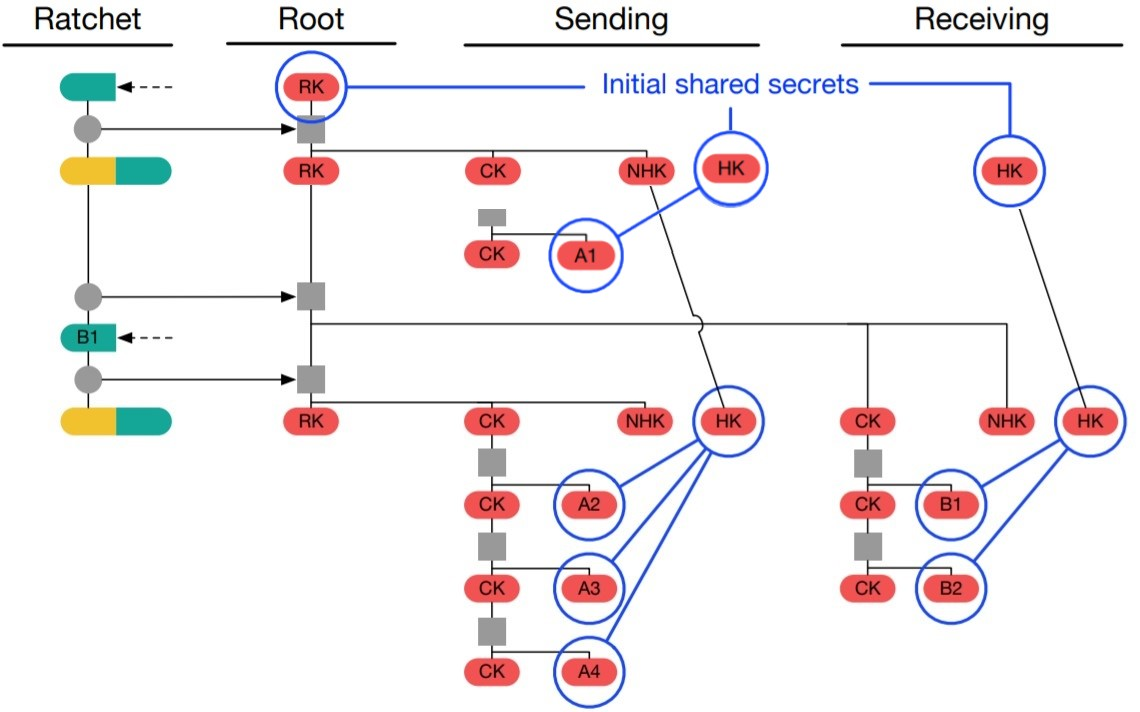
\includegraphics[scale=0.31]{Images/dr-hk.jpg}
	\caption{Usage of \glspl{hk} and \glspl{nhk} in the double ratchet algorithm. Figure reproduced from \cite{dblRtcht}.}
	\label{fig:DR-hk}
\end{figure}

\section{Formal Verification of Signal Protocol}
For completeness, we mention below former work related aimed at formally analyzing the Signal protocol without diving into details.
\par
Cohn-Gordon et al. \cite{cohn2020formal} were the first to address Signal's security in a formal manner. The verification methodology is highly comprehensive and sophisticated, and it is designed particularly for the Signal protocol \cite{alwen_coretti_dodis_2020}. A completely adversarially controlled network is used to evaluate the protocol. Through the definition of a security model, the research covers Signal's \gls{x3dh} and Double Ratchet protocols as a multi-stage authenticated key exchange protocol. The model depicts the ratcheting key update structure as a multi-stage model, where instead of just a sequence, it is a tree-like structure of stages that reflect the chains in Signal. The model enables different parties to run numerous, simultaneous sessions, each with its own set of stages. Secrecy and authentication of message keys in the computational model, under a rich compromise scenario, are the high-level features targeted to be verified by hand. Nevertheless, forward and future secrecy are implied goals, as derived session keys should be kept secret in a range of compromise circumstances. For instance, if a long-term secret is compromised but a medium or ephemeral secret is not, or if a state is compromised and a secure asymmetric stage happens afterwards. Since Signal does not cleanly separate key exchange from subsequent data messages, the model had to reorder some procedures to achieve this separation. In addition and contrary to Signal, the model does not re-use \gls{dh} keys for signatures. Finally, the research shows that Signal's cryptographic core delivers the desirable security attributes specified in the security model, based on normal cryptographic assumptions. Reassuringly, its design is free of any severe defects. The model, on the other hand, fails to explain and address Signal's instantaneous decryption feature, which is a distinctive feature that privileges it to other protocols that lack it \cite{alwen_coretti_dodis_2020}. Furthermore, because the model is exclusive to the Signal protocol, it cannot be used as a reference notion for \gls{rke} because it provides a lower degree of security than would be expected for \gls{rke} \cite{poettering2018asynchronous}.
\par


\section{Post-Quantum Security of Signal Protocol}
The majority of cryptographic primitives are based on mathematical concepts that can be computed and compromised theoretically. These calculations, on the other hand, are computationally challenging. Current cryptographic primitives are robust enough that they cannot be broken by an adversary with typically limited processing capacity. Previously, Shor \cite{shor94} and Grover \cite{gro96} proposed quantum algorithms that, in theory, can infringe the cryptographic principles in a wide range of cryptography primitives.
\par
Shor's algorithm is a quantum computer algorithm for determining an integer's prime factors. The algorithm executes in polynomial time, implying that the integer factorization problem can be performed effectively on a quantum computer. As a result, it could be used to break public-key cryptography schemes like RSA, Finite Field Diffie-Hellman key exchange, and Elliptic Curve Diffie-Hellman key exchange.
\par
Grover's algorithm, commonly known as the quantum search algorithm, is an unstructured search strategy that enhances search performance in unsorted data. When compared to standard counterpart techniques, it results in a quadratic speedup. Grover's algorithm, in the context of cryptography, basically tackles the problem of function inversion. The approach might be used in a variety of symmetric-key cryptography brute-force attacks, including collision and pre-image attacks. For example, it could brute-force a 128-bit symmetric cryptographic key in roughly $ 2^{64} $ iterations, or a 256-bit key in roughly $ 2^{128} $ iterations.
\par
The performance of a quantum computer is substantially superior to that of a regular computer. The security of various cryptographic primitives is jeopardized by the emergence of quantum computers. Hence, if a quantum computer with enough qubits is utilized, all asymmetric cryptography methods and protocols will be broken. On the other hand, If sufficiently high key sizes are used, most symmetric encryption techniques are now deemed quantum-safe \cite{essay77239}. The same may be stated for the majority of hash functions as most of them stay quantum secure \cite{ber09}, given that it is required to create hashes of double the size \cite{bra+98}.
\par

